\section{Results}
Las primeras búsquedas que se realizaron fueron sobre los papers y se quiere lograr una solución en la que cada uno de los bundles contenga artículos relacionados entre sí pero que hayan sido presentados en diferentes conferencias. Separando la búsqueda en los conceptos vistos de Composite Retrieval sería la similitud una función que compara el perfil de cada paper que como vimos anteriormente se obtiene usando los perfiles y la complementaridad el lugar en el cual fue presentado cada paper.\\
Los resultados que aquí se verán son los obtenidos de las ejecuciones de los algoritmos mencionados en ~\cite{compositeRetrival} con las modificaciones propuestas para este trabajo. A continuación se muestran 2 gráficos que reflejan el valor de la función objetivo para los algoritmos BOBO y C-HAC. También se puede observar como mejora la solución cuando se aplica la búsqueda Tabú. Los valores de $\gamma$ que se usaron para los experimentos fueron $0.1$ y $0.9$ pero éstos pueden tomar cualquier valor en el rango $[0:1]$. El mismo sirve para indicar que tipo de soluciones se quieren, a menor valor de $\gamma$ los bundles son mas cohesivos.
\begin{figure}[H]
	\centering
	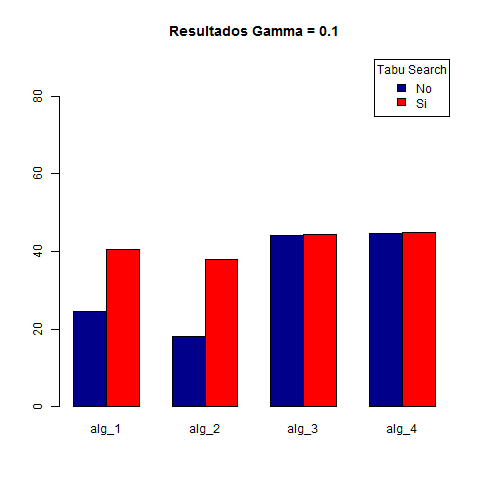
\includegraphics[width=0.25\textwidth]{img/gamma01.png}
	\caption{}
	\label{res:img-gamma01-papers}
\end{figure}

\begin{figure}[H]
	\centering
	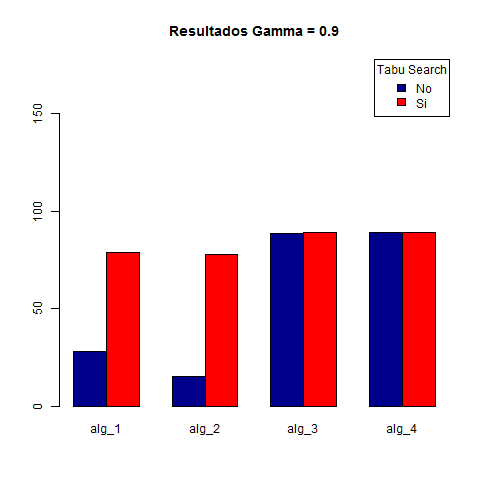
\includegraphics[width=0.25\textwidth]{img/gamma09.png}
	\caption{}
	\label{res:img-gamma09-papers}
\end{figure}
En la segunda búsqueda que se realizo se buscaron bundles de autores los cuáles no sean sean de la misma universidad de afiliación. Como similitud se cuenta con la función que compara el perfil de los autores y como complementaridad la universidad de pertenencia del autor.
\begin{figure}[H]
	\centering
	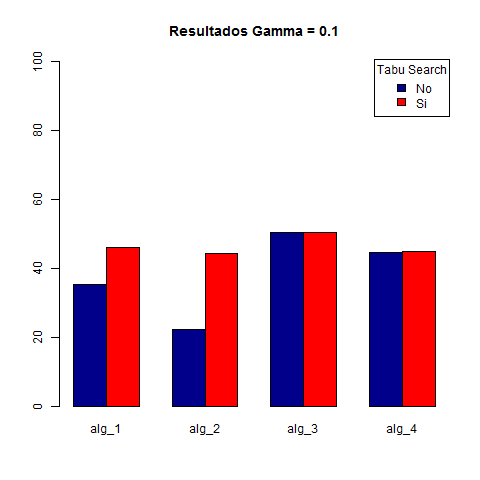
\includegraphics[width=0.25\textwidth]{img/gamma01-autores.png}
	\caption{}
	\label{res:img-gamma01-authors}
\end{figure}

\begin{figure}[H]
	\centering
	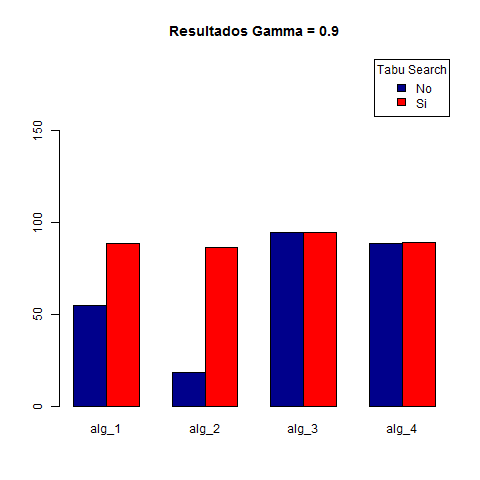
\includegraphics[width=0.25\textwidth]{img/gamma09-autores.png}
	\caption{}
	\label{res:img-gamma09-authors}
\end{figure}
\section{Conclusiones}
Como se ve en los gráficos del punto anterior el uso de la estrategía de búsqueda Tabú funcionó en todos los casos. Para el algoritmo BOBO la mejora fue significativamente mejor y no implicó ningún aumento considerable en el tiempo de ejecución, por lo cuál sin importar el algoritmo usado para generar la solución siempre se debe intentar mejorar mediante la búsqueda Tabú.